\chapter{التنظيم الوظيفي للخلية حقيقية النواة}\label{ch:b1:eukaryotic-cell}

\omterm{def:b1:cell-unit-of-life:cell}{خلية} من البنكرياس تصنع كل يوم ما يقارب كتلتها من الإنزيمات الهاضمة
وتصبها في قناة. والإنزيمات بروتينات كانت لتهضم \omterm{def:b1:cell-unit-of-life:cell}{الخلية} التي صنعتها؛
فهي تبنيها إذن داخل صفيحة غشائية مغلقة، وتشحنها عبر حجيرة ثانية
تُفرز فيها وتُركَّز، وتخزنها في حبيبات، ولا تطلقها إلا عند إشارة
وجبة. وكل خطوة تجري في حيز غشائي مختلف، وتحمل الحويصلات الحركة بين
الأحياز. يصف هذا الفصل حجيرات \omterm{def:b1:cell-unit-of-life:prokeuk}{الخلية حقيقية النواة}، \omterm{def:b1:eukaryotic-cell:endomembrane}{والجملة الغشائية
الداخلية} التي تجري فيها البروتينات، \omterm{def:b1:cell-unit-of-life:prokeuk}{والعضيات} التي تحول الطاقة،
والهيكل الذي يمسك شكل \omterm{def:b1:cell-unit-of-life:cell}{الخلية} ويحرك أجزاءها، والخصائص التي تميز \omterm{def:b1:cell-unit-of-life:cell}{خلية}
نباتية من \omterm{def:b1:cell-unit-of-life:cell}{خلية} حيوانية.

\section{الحجيرات}

\begin{definition}[العضية والعصارة الخلوية]\label{def:b1:eukaryotic-cell:organelle}
\emph{العضية}\index{عضية} بنية داخل \omterm{def:b1:cell-unit-of-life:cell}{الخلية} لها تركيب محدد ووظيفة
محددة؛ \omterm{def:b1:cell-unit-of-life:prokeuk}{والعضيات} المحدودة بأغشية حجيرات يختلف داخلها في تركيبه عن
\emph{العصارة الخلوية}\index{عصارة خلوية}، وهي المحلول المائي
\omterm{def:b1:cell-unit-of-life:cell}{للسيتوبلازم} خارجها. والحجيرات المحدودة بأغشية هي: \omterm{def:b1:eukaryotic-cell:nucleus}{النواة}، \omterm{def:b1:eukaryotic-cell:endomembrane}{والشبكة
الإندوبلازمية}، \omterm{def:b1:eukaryotic-cell:endomembrane}{وجهاز غولجي}، \omterm{def:b1:eukaryotic-cell:endomembrane}{والجسيمات الحالة}، \omterm{def:b1:eukaryotic-cell:peroxisome}{والبيروكسيسومات}،
\omterm{def:b1:eukaryotic-cell:mitochondrion}{والمتقدرات}، \omterm{def:b1:eukaryotic-cell:plastid}{والبلاستيدات} \omterm{def:b1:eukaryotic-cell:plantcell}{والفجوة} في النبات. \omterm{def:b1:cell-unit-of-life:prokeuk}{والعضيات} بلا غشاء هي:
الريبوزومات، \omterm{def:b1:eukaryotic-cell:cytoskeleton}{والجسيم المركزي}، \omterm{def:b1:eukaryotic-cell:cytoskeleton}{والهيكل الخلوي}.
\end{definition}

\begin{omfigure}
\begin{tikzpicture}
  \node[anchor=south west, inner sep=0] (img) at (0,0)
    {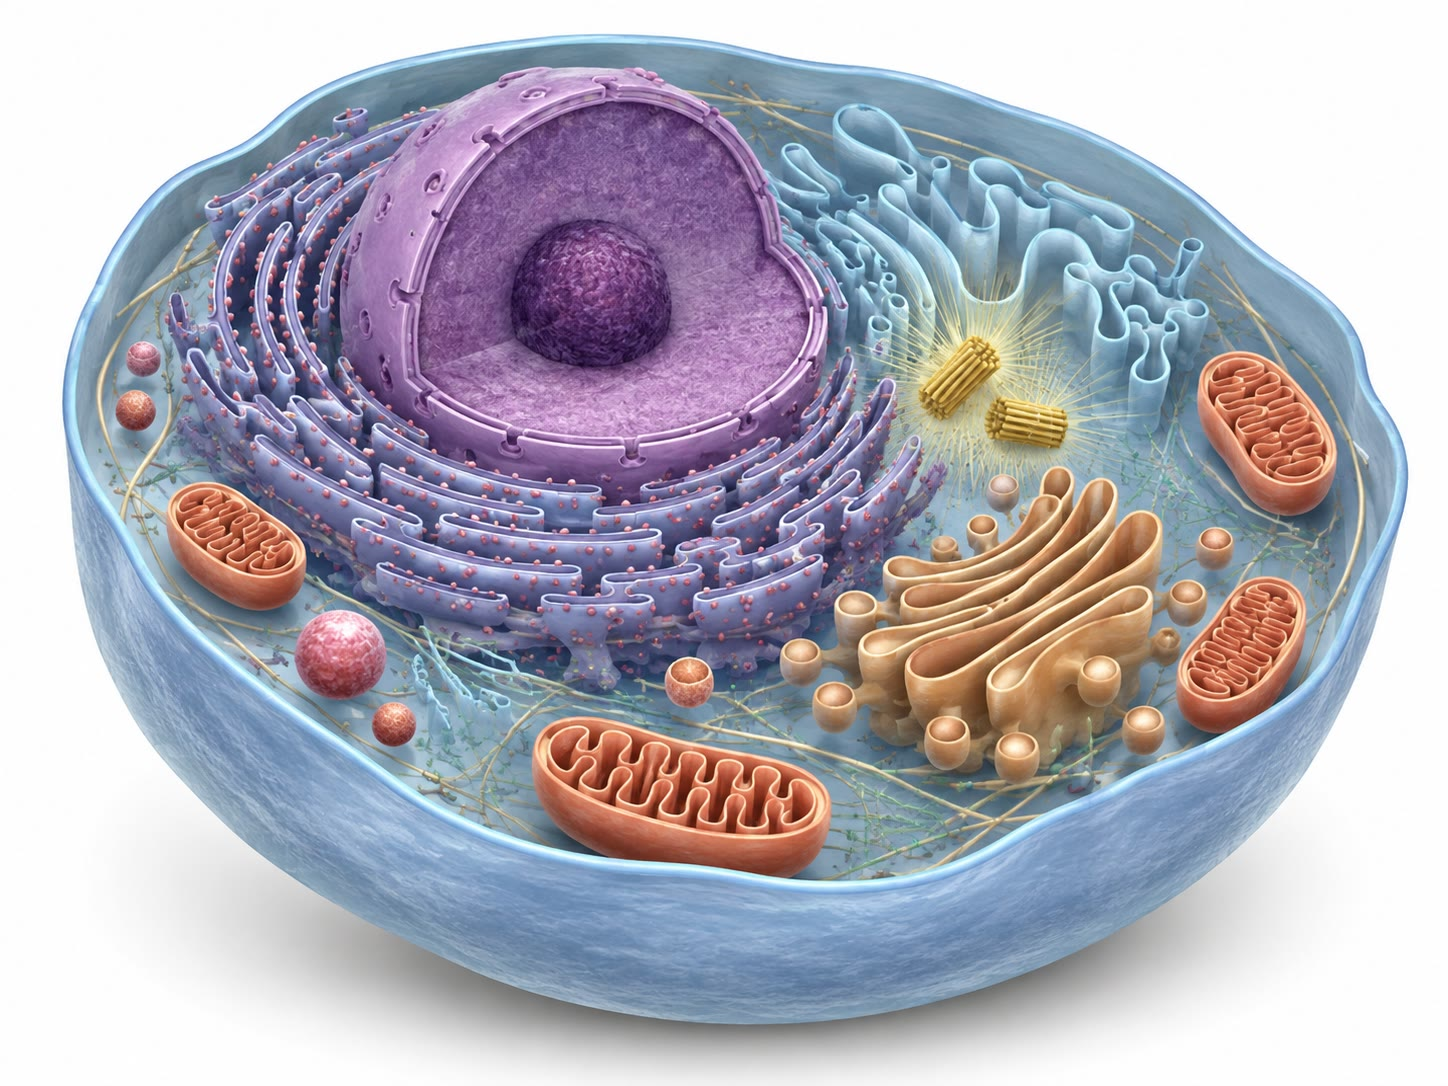
\includegraphics[width=0.6\linewidth]{images/book3/ai/fig-animal-cell-cutaway.jpg}};
  \begin{scope}[x={(img.south east)}, y={(img.north west)},
      every node/.style={font=\small}]
    \draw[omDef, thick] (0.42,0.72) -- (0.42,1.08) node[above] {نواة، ونوية، وثقوب};
    \draw[omDef, thick] (0.30,0.52) -- (-0.03,0.44) node[left, align=right] {شبكة إندوبلازمية\\ خشنة};
    \draw[omDef, thick] (0.23,0.42) -- (-0.03,0.22) node[left] {جسيم حال};
    \draw[omDef, thick] (0.07,0.62) -- (-0.03,0.76) node[left] {غشاء بلازمي};
    \draw[omDef, thick] (0.75,0.80) -- (1.03,0.88) node[right] {شبكة ملساء};
    \draw[omDef, thick] (0.69,0.63) -- (1.03,0.62) node[right] {جسيم مركزي};
    \draw[omDef, thick] (0.87,0.42) -- (1.03,0.36) node[right] {متقدرة};
    \draw[omDef, thick] (0.70,0.40) -- (0.80,-0.08) node[below] {جهاز غولجي وحويصلاته};
    \draw[omDef, thick] (0.47,0.25) -- (0.35,-0.08) node[below] {متقدرة};
  \end{scope}
\end{tikzpicture}

{\small \omterm{def:b1:cell-unit-of-life:cell}{خلية} حيوانية معممة مشقوقة. \omterm{def:b1:eukaryotic-cell:nucleus}{النواة} في المركز؛ وحولها \omterm{def:b1:eukaryotic-cell:endomembrane}{الشبكة
الإندوبلازمية الخشنة} المتصلة \omterm{def:b1:eukaryotic-cell:nucleus}{بالغلاف النووي}، والشبكة الملساء، وكدس
غولجي وحويصلاته، \omterm{def:b1:eukaryotic-cell:mitochondrion}{والمتقدرات}، \omterm{def:b1:eukaryotic-cell:endomembrane}{والجسيمات الحالة}، \omterm{def:b1:eukaryotic-cell:cytoskeleton}{والجسيم المركزي} الذي
تشع منه \omterm{def:b1:eukaryotic-cell:cytoskeleton}{الأنيبيبات الدقيقة}.}
\end{omfigure}

\begin{definition}[النواة]\label{def:b1:eukaryotic-cell:nucleus}
تحفظ \emph{النواة}\index{نواة} الصبغيات في هيئة
\emph{صبغين}\index{صبغين}، وهو DNA ملفوف على بروتينات هستونية
(\cref{ch:b1:genomes}). ويحدها \emph{الغلاف النووي}\index{غلاف نووي}،
وهو غشاءان، الخارجي منهما متصل \omterm{def:b1:eukaryotic-cell:endomembrane}{بالشبكة الإندوبلازمية}، مثقوب
\emph{بثقوب نووية}\index{ثقب نووي} يعبرها RNA والبروتينات في
الاتجاهين تحت تحكم. و\emph{النوية}\index{نوية} هي المنطقة التي يُصنع
فيها RNA الريبوزومي وتُركَّب فيها الريبوزومات. والنواة تفصل الاستنساخ
(في الداخل) عن الترجمة (في الخارج)، وهو فصل لا تملكه \omterm{def:b1:cell-unit-of-life:prokeuk}{بدائيات النواة}.
\end{definition}

\begin{proposition}[حجيرات خلية كبدية]\label{prop:b1:eukaryotic-cell:budget}
في \omterm{def:b1:cell-unit-of-life:cell}{خلية} كبدية حجمها \qty{5000}{\micro m^3}، تأخذ \omterm{def:b1:eukaryotic-cell:organelle}{العصارة الخلوية} نحو
نصف الحجم، \omterm{def:b1:eukaryotic-cell:mitochondrion}{والمتقدرات} خمسه، \omterm{def:b1:eukaryotic-cell:endomembrane}{والشبكة الإندوبلازمية} سدسه، \omterm{def:b1:eukaryotic-cell:nucleus}{والنواة} جزءًا
من ستة عشر، \omterm{def:b1:eukaryotic-cell:endomembrane}{وجهاز غولجي} \omterm{def:b1:eukaryotic-cell:endomembrane}{والجسيمات الحالة} \omterm{def:b1:eukaryotic-cell:peroxisome}{والبيروكسيسومات} بضعة في
المئة معًا. أما الأغشية فتحكي حكاية أخرى: فمن \qty{110000}{\micro m^2}
من الغشاء في \omterm{def:b1:cell-unit-of-life:cell}{الخلية}، نصفها \omterm{def:b1:eukaryotic-cell:endomembrane}{شبكة إندوبلازمية}، وثلثها الغشاء الداخلي
\omterm{def:b1:eukaryotic-cell:mitochondrion}{للمتقدرات}، و\qty{2}{\%} فقط الغشاء البلازمي. فمعظم غشاء \omterm{def:b1:cell-unit-of-life:cell}{الخلية} في
داخلها.
\end{proposition}

\begin{omfigure}
\begin{tikzpicture}
\begin{axis}[
  xbar, bar width=8pt,
  width=0.72\linewidth, height=6.4cm,
  axis x line=bottom, axis y line=left,
  xmin=0, xmax=45, xlabel={النصيب من مجموع غشاء الخلية (\%)},
  xlabel style={font=\small, at={(axis description cs:0.5,-0.13)}, anchor=north},
  symbolic y coords={الغلاف النووي, الغشاء البلازمي, الجسيمات الحالة والبيروكسيسومات, جهاز غولجي, الغشاء المتقدري الخارجي, الشبكة الملساء, الغشاء المتقدري الداخلي, الشبكة الخشنة},
  ytick=data, tick label style={font=\small},
  enlarge y limits=0.08, xtick={0,10,20,30,40},
  nodes near coords, nodes near coords style={font=\scriptsize, anchor=west},
]
\addplot[fill=omDef!45, draw=omDef] coordinates
  {(0.2,الغلاف النووي) (2,الغشاء البلازمي) (1.5,الجسيمات الحالة والبيروكسيسومات) (7,جهاز غولجي) (7,الغشاء المتقدري الخارجي) (16,الشبكة الملساء) (32,الغشاء المتقدري الداخلي) (35,الشبكة الخشنة)};
\end{axis}
\end{tikzpicture}

{\small أين يقع غشاء \omterm{def:b1:cell-unit-of-life:cell}{خلية} كبدية. الغشاء البلازمي، وهو الوحيد المرئي
من الخارج، اثنان في المئة من المجموع؛ والشبكة والغشاء المتقدري
الداخلي، المطويان في الداخل، أربعة أخماسه.}
\end{omfigure}

\section{الجملة الغشائية الداخلية}

\begin{definition}[الشبكة الإندوبلازمية وجهاز غولجي والجسيم الحال]\label{def:b1:eukaryotic-cell:endomembrane}
\emph{الشبكة الإندوبلازمية}\index{شبكة إندوبلازمية} شبكة من صفائح
وأنابيب غشائية تحيط بحيز واحد متصل هو اللمعة، وهي متصلة \omterm{def:b1:eukaryotic-cell:nucleus}{بالغلاف
النووي}. وجزؤها \emph{الخشن}\index{شبكة إندوبلازمية خشنة} مرصع
بريبوزومات تحقن ما تصنعه من بروتينات في اللمعة أو في الغشاء؛ وجزؤها
\emph{الأملس}\index{شبكة إندوبلازمية ملساء} يصنع الدهون، ويخزن
الكالسيوم، ويزيل السموم. و\emph{جهاز غولجي}\index{جهاز غولجي} كدس من
أكياس مفلطحة (صهاريج)، له وجه \emph{قريب} مستقبِل قرب الشبكة ووجه
\emph{بعيد} شاحن، تُعدَّل فيه البروتينات الآتية من الشبكة (فتُقلَّم
السكريات وتُضاف)، وتُفرز، وتُعبَّأ في حويصلات إلى وجهاتها.
و\emph{الجسيمات الحالة}\index{جسيم حال} حويصلات حمضية
(pH $\approx 5$) مملوءة بإنزيمات حالة تهضم ما يُدخل من الخارج أو
\omterm{def:b1:cell-unit-of-life:prokeuk}{العضيات} البالية. وهذه، مع الحويصلات المتنقلة بينها وبين الغشاء
البلازمي، تكوّن \emph{الجملة الغشائية الداخلية}\index{الجملة الغشائية الداخلية}:
وهي مجموعة حجيرات متصلة، لمعاتها من حيث الطوبولوجيا هي خارج \omterm{def:b1:cell-unit-of-life:cell}{الخلية}.
\end{definition}

\begin{proposition}[السبيل الإفرازي]\label{prop:b1:eukaryotic-cell:secretory}
\index{السبيل الإفرازي}
البروتين المعدّ للإفراز، أو للغشاء البلازمي، أو \omterm{def:b1:eukaryotic-cell:endomembrane}{لجسيم حال}، تصنعه
ريبوزومات مرتبطة بالشبكة الخشنة، ويدخل لمعة الشبكة وهو يُصنع، ويلتف
فيها، ثم يسافر في حويصلات إلى الوجه القريب من غولجي، ويعبر الكدس
وهو يُعدَّل، ويغادر الوجه البعيد في حويصلة معنونة إلى وجهتها:
حبيبة إفرازية تندمج بالغشاء البلازمي عند إشارة (\emph{إخراج خلوي
منظَّم}\index{إخراج خلوي})، أو حويصلة تندمج باستمرار (\omterm{prop:b1:eukaryotic-cell:secretory}{إخراج خلوي}
\emph{بنيوي}، وهو يوصل أيضًا غشاءً جديدًا)، أو \omterm{def:b1:eukaryotic-cell:endomembrane}{جسيم حال}. أما
البروتينات العصارية والنووية فتُصنع على ريبوزومات حرة ولا تدخل
الجملة قط. والذي يحسم الأمر هو \emph{تسلسل إشارة}\index{تسلسل إشارة}
في أول البروتين (\cref{ch:b1:gene-expression}).
\end{proposition}
\begin{proof}[شواهد]
أطعم بالادِه (ستينيات القرن العشرين) شرائح من بنكرياس خنزير غينيا
حموضًا أمينية مشعة ثلاث دقائق (\emph{النبضة})، ثم حموضًا غير مشعة
(\emph{الملاحقة})، ثم حدد موضع الإشعاع بالتصوير الإشعاعي الذاتي
لصور مجهرية إلكترونية على فترات. فعند \qty{3}{min} كانت حبيبات
الفضة فوق الشبكة الخشنة؛ وعند \qty{20}{min} فوق غولجي؛ وعند
\qty{40}{min} فوق فجوات مكثِّفة وحبيبات جديدة؛ وعند \qty{2}{h} في
لمعة القناة. وأعطت \omterm{def:b1:cell-unit-of-life:fractionation}{تجزئة الخلايا} التتابع نفسه كيميائيًا. ثم بيّن
بلوبل (سبعينيات القرن العشرين) أن البروتينات المفرزة المصنوعة في
أنبوب اختبار بلا أغشية تزيد عشرين بقية عن الصورة المفرزة ولا تُحمى من
بروتياز مضاف، بينما تُشطر وتُحمى إذا صُنعت بوجود أغشية الشبكة:
فالبقايا الزائدة هي الإشارة التي توجه السلسلة النامية إلى الشبكة.
\end{proof}

\begin{omfigure}
\begin{tikzpicture}
\begin{axis}[
  width=0.9\linewidth, height=6.2cm,
  axis x line=bottom, axis y line=left,
  xmin=0, xmax=130, ymin=0, ymax=105,
  xlabel={الزمن بعد النبضة (min)}, ylabel={النصيب من الوسم (\%)},
  xlabel style={font=\small, at={(axis description cs:0.5,-0.12)}, anchor=north},
  ylabel style={font=\small},
  tick label style={font=\small}, xtick={0,20,40,60,80,100,120}, ytick={0,25,50,75,100},
  legend style={font=\small, at={(0.5,-0.24)}, anchor=north, draw=none, legend columns=2, /tikz/every even column/.append style={column sep=0.4cm}},
  clip=false,
]
\addplot[very thick, omDef, smooth] coordinates {(3,88) (7,55) (15,25) (30,8) (60,2) (120,0)};
\addlegendentry{الشبكة الخشنة}
\addplot[very thick, omProp, smooth] coordinates {(3,8) (7,35) (15,55) (30,35) (60,10) (120,2)};
\addlegendentry{غولجي والفجوات المكثِّفة}
\addplot[very thick, omThm, smooth] coordinates {(3,0) (7,3) (15,12) (30,45) (60,70) (90,55) (120,30)};
\addlegendentry{الحبيبات الإفرازية}
\addplot[very thick, omExo, smooth] coordinates {(3,0) (7,0) (15,0) (30,2) (60,12) (90,35) (120,65)};
\addlegendentry{المفرَز في القناة}
\end{axis}
\end{tikzpicture}

{\small نبضة بالادِه وملاحقتها في البنكرياس: أين تقع البروتينات
الموسومة بدلالة الزمن. فهي تنتقل من الشبكة إلى غولجي في ربع ساعة،
وتبلغ الحبيبات في غضون الساعة، وتغادر \omterm{def:b1:cell-unit-of-life:cell}{الخلية} في الساعتين التاليتين.}
\end{omfigure}

\begin{omfigure}
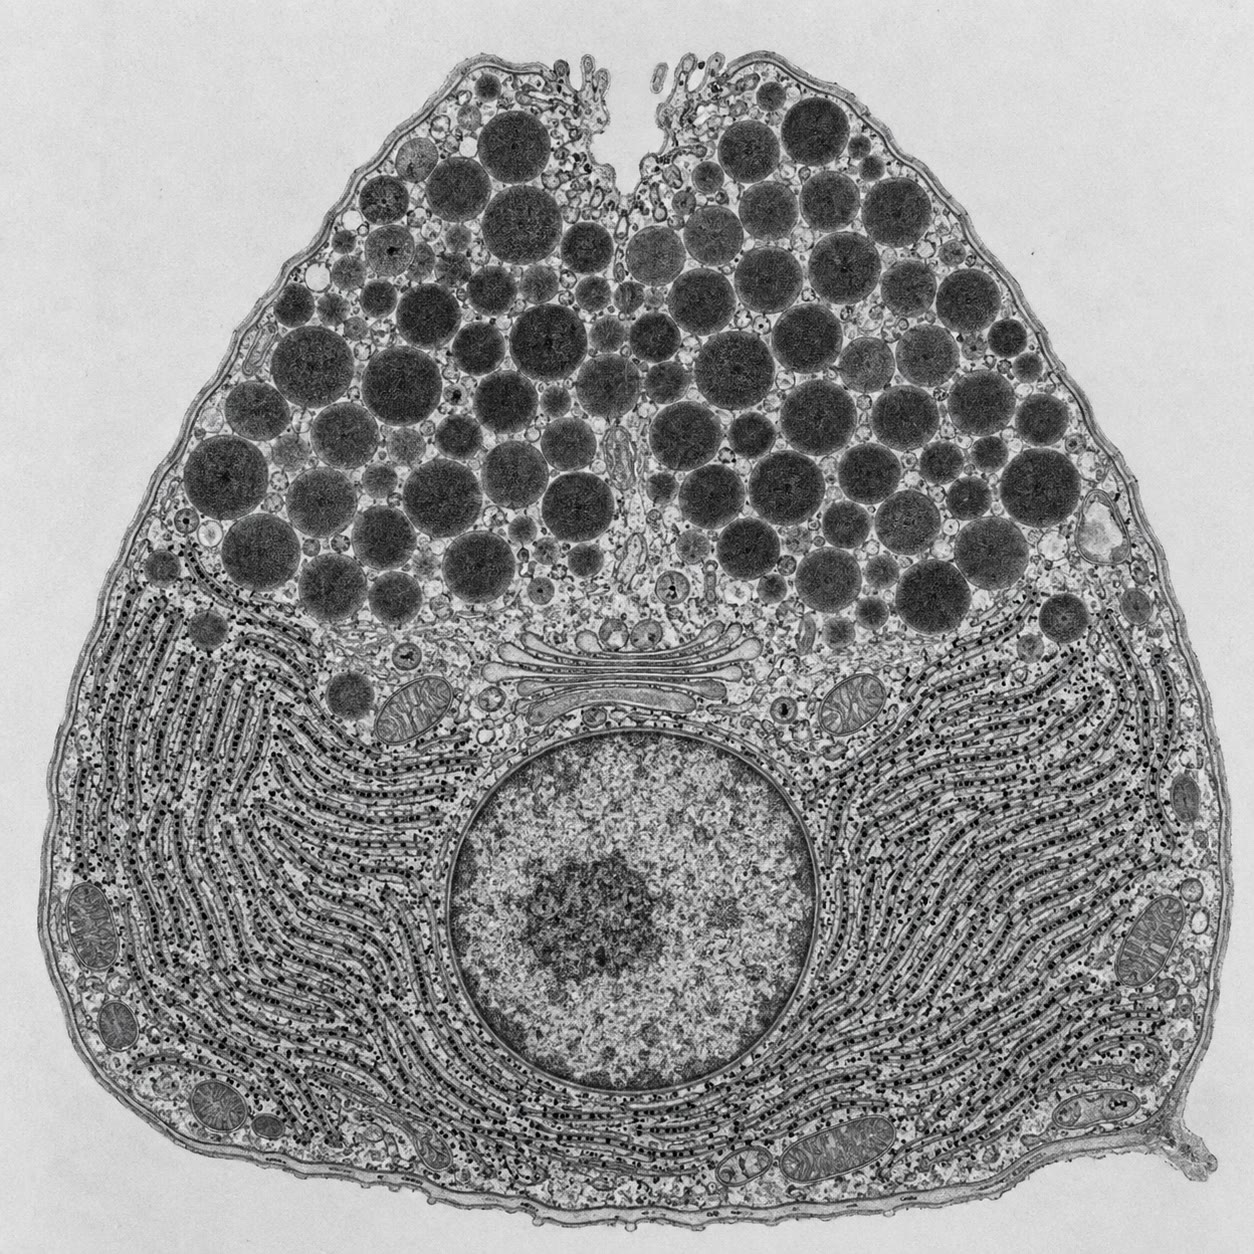
\includegraphics[width=0.44\linewidth]{images/book3/ai/b3-06-acinar-cell-tem.jpg}

{\small \omterm{def:b1:cell-unit-of-life:cell}{خلية} عنبية بنكرياسية في \omterm{prop:b1:cell-unit-of-life:microscopes}{المجهر الإلكتروني} النافذ: شبكة خشنة
مرصوصة أكداسًا متوازية حول \omterm{def:b1:eukaryotic-cell:nucleus}{النواة} عند القاعدة، وغولجي فوقها،
والحبيبات الإفرازية الكثيفة محتشدة نحو القمة والقناة.}
\end{omfigure}

\begin{method}[تتبع جزيء عبر الخلية]\label{met:b1:eukaryotic-cell:pulsechase}
\begin{enumerate}
  \item وسّم فوجًا قصيرًا: عرّض \omterm{def:b1:cell-unit-of-life:cell}{الخلايا} لطليعة مشعة أو متألقة بضع
        دقائق (النبضة)، ثم استبدل بها فائضًا من الطليعة غير الموسومة
        (الملاحقة)، حتى لا يحمل الوسم إلا الجزيئات المصنوعة في أثناء
        النبضة.
  \item خذ عينات على فترات، وثبّتها، وحدد موضع الوسم: بالتصوير
        الإشعاعي الذاتي للمقاطع، أو بالمجهرية التألقية، أو بالتجزئة
        والعد.
  \item الحجيرة التي يبلغ وسمها ذروته أولًا هي الأعلى في المجرى؛
        وتتابع الذُّرى هو المسار؛ والفواصل هي أزمنة العبور.
  \item اسدد خطوة (بالبرد، أو بمثبط للطاقة، أو بطافرة) وانظر أين
        يتراكم الوسم: فهو في الحجيرة السابقة للسد.
\end{enumerate}
\end{method}

\begin{definition}[الإدخال الخلوي]\label{def:b1:eukaryotic-cell:endocytosis}
\emph{الإدخال الخلوي}\index{إدخال خلوي} يجلب المواد إلى الداخل:
فينثني الغشاء البلازمي حولها ويقرص حويصلة تندمج عادة \omterm{def:b1:eukaryotic-cell:endomembrane}{بجسيم حال}.
و\emph{البلعمة} تبتلع الجسيمات (بكتيريا، أو \omterm{def:b1:cell-unit-of-life:cell}{خلية} ميتة)؛
و\emph{الاحتساء} يأخذ قطيرات من السائل؛ و\emph{الإدخال الخلوي
بوساطة المستقبِلات} يركّز جزيئًا بعينه (جسيمات حاملة للكولستيرول،
والترانسفيرين الحامل للحديد) على مستقبِلات في حفر مغلفة قبل إدخاله.
\omterm{prop:b1:eukaryotic-cell:secretory}{والإخراج الخلوي} يضيف غشاءً إلى سطح \omterm{def:b1:cell-unit-of-life:cell}{الخلية} والإدخال ينزعه؛ وفي \omterm{def:b1:cell-unit-of-life:cell}{خلية}
مفرزة يتوازن الاثنان فيبقى السطح ثابتًا بينما تدور عبره مساحات
كاملة من الغشاء كل ساعة.
\end{definition}

\section{المتقدرات والبلاستيدات}

\begin{definition}[المتقدرة]\label{def:b1:eukaryotic-cell:mitochondrion}
\emph{المتقدرة}\index{متقدرة} \omterm{def:b1:eukaryotic-cell:organelle}{عضية} عرضها
\qtyrange{0.5}{1}{\micro m} وطولها بضعة ميكرومترات، يحدها غشاءان:
غشاء خارجي أملس ينفذ للجزيئات الصغيرة، وغشاء داخلي مطوي إلى
\emph{أعراف}\index{عرف} لا ينفذ للشوارد ويحمل سلسلة التنفس وسنتاز
ATP (\cref{ch:b1:respiration-fermentation}). وفي الداخل
\emph{الحشوة}\index{حشوة المتقدرة}، وهي تحمل إنزيمات دورة كريبس،
وريبوزومات من الطراز البكتيري، وعدة نسخ من DNA حلقي صغير. والمتقدرات
تنقسم بالانشطار، وتتحرك على \omterm{def:b1:eukaryotic-cell:cytoskeleton}{الهيكل الخلوي}، ويتراوح عددها بين بضع مئات
وبضعة آلاف في \omterm{def:b1:cell-unit-of-life:cell}{الخلية}.
\end{definition}

\begin{definition}[البلاستيدات]\label{def:b1:eukaryotic-cell:plastid}
\emph{البلاستيدات}\index{بلاستيدة} هي \omterm{def:b1:cell-unit-of-life:prokeuk}{عضيات} \omterm{def:b1:cell-unit-of-life:cell}{الخلية} النباتية ذات
الغشاء المضاعف: \emph{البلاستيدات الخضراء}\index{بلاستيدة خضراء}،
التي تجري فيها جملة ثالثة من الأغشية، هي
\emph{الثايلاكويدات}\index{ثايلاكويد} المكدسة في أكداس والمغمورة في
\emph{السدى}\index{سدى}، التركيب الضوئي
(\cref{ch:b1:photosynthesis})؛ والبلاستيدات النشوية، التي تدخر
النشا؛ والبلاستيدات الملونة، التي تحمل أصبغة الثمار والبتلات. وكلها
مشتقة من بلاستيدات أولية، وهي، مثل \omterm{def:b1:eukaryotic-cell:mitochondrion}{المتقدرات}، تحوي DNA حلقيًا خاصًا
بها وريبوزومات من الطراز البكتيري وتنقسم بالانشطار.
\end{definition}

\begin{omfigure}
\begin{minipage}[b]{0.48\linewidth}\centering
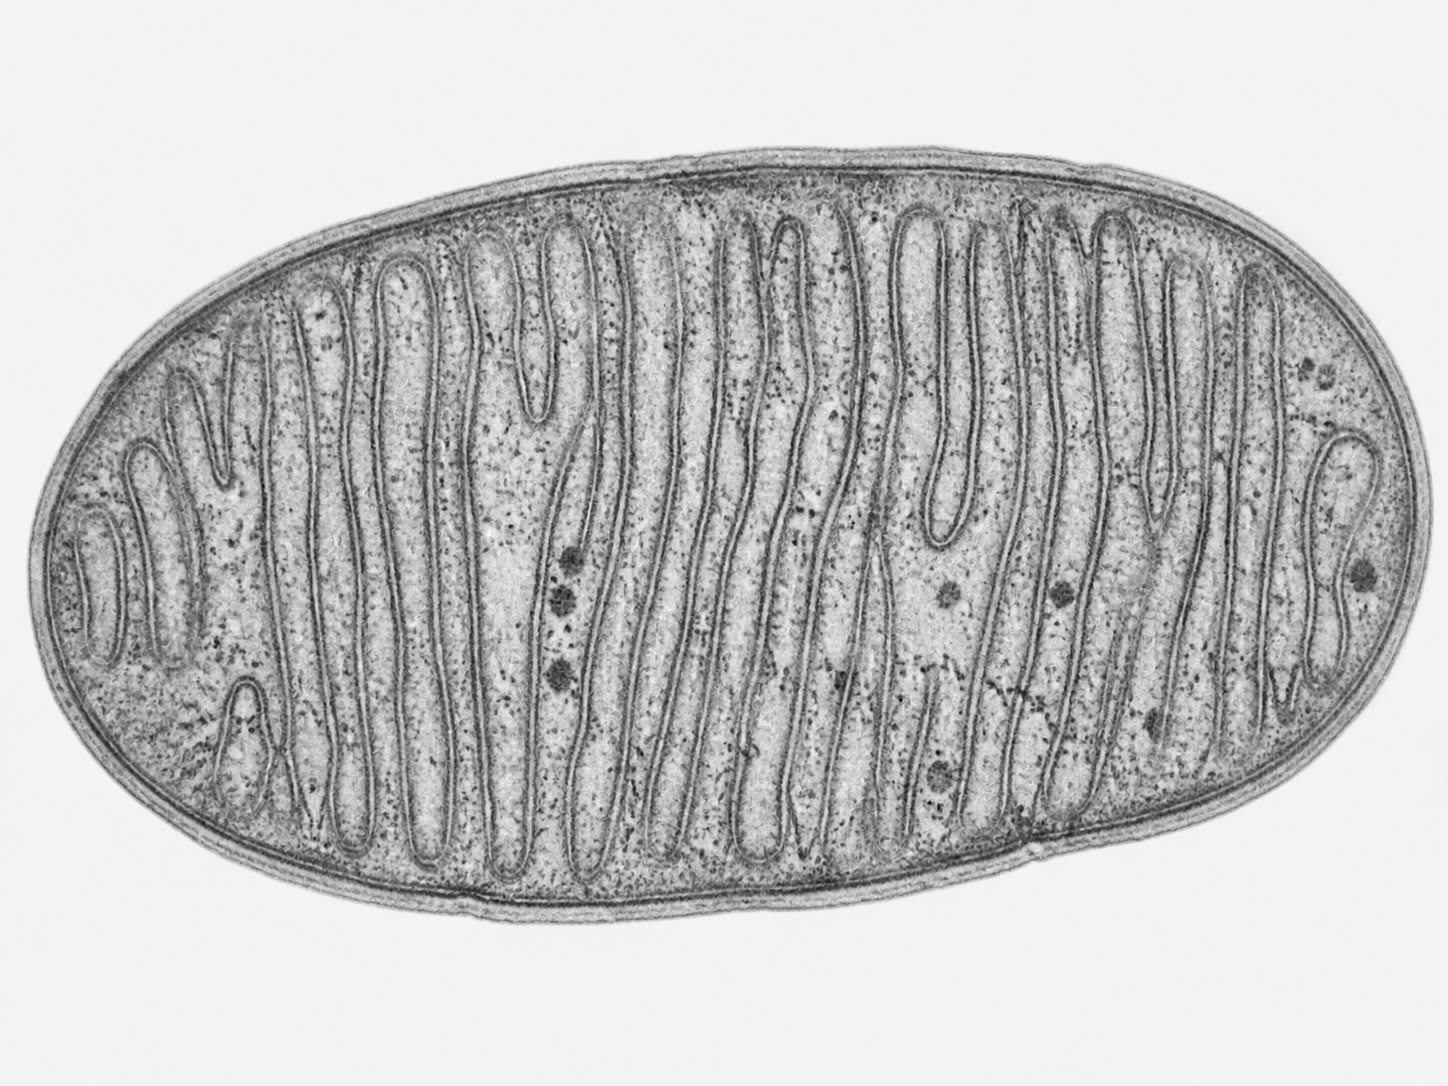
\includegraphics[width=0.96\linewidth]{images/book2/ai/g12-resp-mitochondrion-tem.jpg}
\end{minipage}\hfill
\begin{minipage}[b]{0.48\linewidth}\centering
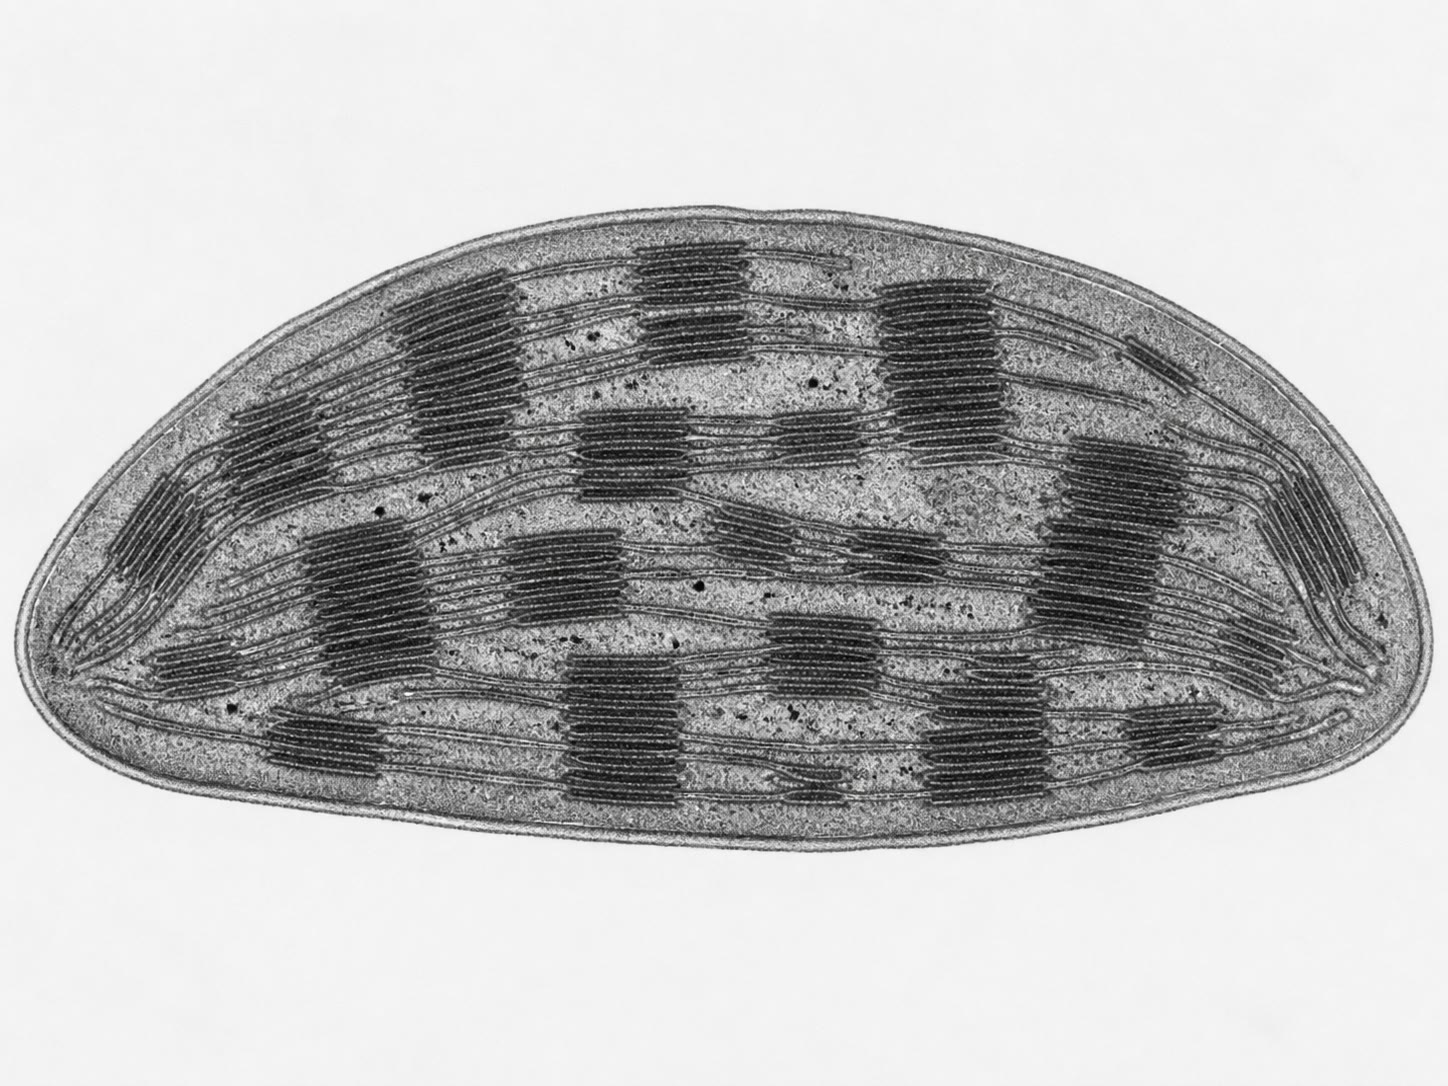
\includegraphics[width=0.96\linewidth]{images/book2/ai/g12-photo-chloroplast-tem.jpg}
\end{minipage}

{\small \omterm{def:b1:eukaryotic-cell:mitochondrion}{متقدرة} (إلى اليسار) \omterm{def:b1:eukaryotic-cell:plastid}{وبلاستيدة خضراء} (إلى اليمين) في مقطع تحت
\omterm{prop:b1:cell-unit-of-life:microscopes}{المجهر الإلكتروني}. لكل منهما غشاءا غلاف؛ وفي الداخل الغشاء الداخلي
المطوي عند \omterm{def:b1:eukaryotic-cell:mitochondrion}{المتقدرة} \omterm{def:b1:eukaryotic-cell:plastid}{والثايلاكويدات} المكدسة عند \omterm{def:b1:eukaryotic-cell:plastid}{البلاستيدة} --- وهي
الأغشية التي تُحوَّل عليها الطاقة.}
\end{omfigure}

\begin{proposition}[الأصل التعايشي الداخلي]\label{prop:b1:eukaryotic-cell:endosymbiosis}
\index{التعايش الداخلي}
تنحدر \omterm{def:b1:eukaryotic-cell:mitochondrion}{المتقدرات} \omterm{def:b1:eukaryotic-cell:plastid}{والبلاستيدات} من بكتيريا حرة المعيشة ابتلعتها \omterm{def:b1:cell-unit-of-life:prokeuk}{خلية
حقيقية النواة} سلف واحتفظت بها متعايشة: \omterm{def:b1:eukaryotic-cell:mitochondrion}{فالمتقدرات} من بكتيريا هوائية،
\omterm{def:b1:eukaryotic-cell:plastid}{والبلاستيدات} من بكتيريا زرقاء.
\end{proposition}
\begin{proof}[شواهد]
لكلتا العضيتين غشاءان، الداخلي منهما بتركيب بكتيري والخارجي يشبه
غشاء المضيف؛ وصبغي حلقي بلا هستونات؛ وريبوزومات بالقياس البكتيري
وبحساسيته للمضادات الحيوية؛ وشيفرة وراثية بمتغيرات بكتيرية؛ وانقسام
ثنائي مستقل عن انقسام \omterm{def:b1:cell-unit-of-life:cell}{الخلية}؛ ومورّثاتها، حين تُقرأ تسلسلاتها،
تنتظم مع مورّثات أنساب بكتيرية بعينها (ألفا بروتيوبكتيريا، وبكتيريا
زرقاء) لا مع المورّثات النووية \omterm{def:b1:cell-unit-of-life:cell}{للخلية} التي تؤويها. وقد انتقل معظم
مورّثاتها الأصلية منذ ذلك الحين إلى \omterm{def:b1:eukaryotic-cell:nucleus}{النواة}، ولم تعد العضيتان تقدران
على العيش وحدهما.
\end{proof}

\begin{definition}[البيروكسيسوم]\label{def:b1:eukaryotic-cell:peroxisome}
\emph{البيروكسيسوم}\index{بيروكسيسوم} \omterm{def:b1:eukaryotic-cell:organelle}{عضية} صغيرة ذات غشاء وحيد تحوي
إنزيمات مؤكسدة تنقل الهيدروجين من ركائز (حموض دسمة، كحول) إلى
الأكسجين، فتنتج ماءً أكسجينيًا، وتحوي الكاتالاز الذي يهدم الماء
الأكسجيني في مكانه. فهي تحصر كيمياء خطرة.
\end{definition}

\section{الهيكل الخلوي}

\begin{definition}[الهيكل الخلوي]\label{def:b1:eukaryotic-cell:cytoskeleton}
\emph{الهيكل الخلوي}\index{هيكل خلوي} شبكة من الخيوط البروتينية تمنح
\omterm{def:b1:cell-unit-of-life:cell}{الخلية} شكلها، وترسّي عضياتها، وتحركها وتحرك \omterm{def:b1:cell-unit-of-life:cell}{الخلية} نفسها. وهو ثلاثة
أنواع: \emph{الخييطات الدقيقة}\index{خييط دقيق} من الأكتين
(\qty{7}{nm}، خصلتان ملتويتان من وحيدات كروية)، وهي متركزة تحت
الغشاء البلازمي، ومسؤولة عن شكل \omterm{def:b1:cell-unit-of-life:cell}{الخلية}، والزحف، وحلقة الانقسام
المتقلصة، والتقلص العضلي مع الميوزين؛
و\emph{الأنيبيبات الدقيقة}\index{أنيبيب دقيق} (أنابيب جوفاء قطرها
\qty{25}{nm} من التوبيولين)، وهي تشع من \emph{الجسيم
المركزي}\index{جسيم مركزي}، وتكون مسارات تحمل عليها البروتينات
المحركة (الكينيزين إلى الخارج والداينين إلى الداخل) الحويصلات
\omterm{def:b1:cell-unit-of-life:prokeuk}{والعضيات}، وتكوّن مغزل الانقسام ولب الأهداب والأسواط؛
و\emph{الخيوط المتوسطة}\index{خيط متوسط} (\qty{10}{nm}، شبيهة
بالحبال، من الكيراتينات وما يقاربها)، وهي الألياف المقاومة ميكانيكيًا
التي تصلّب \omterm{def:b1:cell-unit-of-life:cell}{الخلايا} وترسو عند الجسيمات الرابطة. والخييطات الدقيقة
والأنيبيبات الدقيقة تتجمع وتتفكك باستمرار من مخزون وحيداتها.
\end{definition}

\begin{omfigure}
\begin{tikzpicture}[font=\footnotesize, line cap=round]
  % actin: two twisted strands of beads
  \foreach \i in {0,...,15} {
    \pgfmathsetmacro{\y}{0.13*sin(\i*45)}
    \fill[omThm!70] (0.35*\i,1.6+\y) circle (0.11);
    \fill[omThm!45] (0.35*\i+0.17,1.6-\y) circle (0.11);
  }
  \node[anchor=west, align=left] at (6.0,1.6) {\textbf{خييط دقيق} (أكتين)، \qty{7}{nm}\\ الشكل، والزحف، وحلقة الانقسام، والعضل};
  % intermediate filament: rope of coiled strands
  \foreach \k in {0,1,2,3} {
    \draw[omProp, thick] plot[domain=0:5.3, samples=60] (\x, {0.55+0.09*sin(180*\x+90*\k)});
  }
  \node[anchor=west, align=left] at (6.0,0.55) {\textbf{خيط متوسط}، \qty{10}{nm}\\ شبيه بالحبل، للمتانة الميكانيكية};
  % microtubule: hollow tube of protofilaments
  \draw[thick, omDef!70!black, fill=omDef!15] (0,-0.9) rectangle (5.3,-0.2);
  \foreach \i in {0,...,25} { \foreach \j in {0,1,2,3} {
    \fill[omDef!60] (0.1+0.2*\i, -0.83+0.19*\j) circle (0.075);
  } }
  \draw[thick, omDef!70!black, fill=omDef!10] (5.3,-0.55) ellipse (0.18 and 0.35);
  \draw[thick, omDef!70!black, fill=white] (5.3,-0.55) ellipse (0.10 and 0.24);
  \node[anchor=west, align=left] at (6.0,-0.55) {\textbf{أنيبيب دقيق} (توبيولين)، \qty{25}{nm} أجوف\\ مسارات للمحركات، والمغزل، والأهداب};
\end{tikzpicture}

{\small خيوط \omterm{def:b1:eukaryotic-cell:cytoskeleton}{الهيكل الخلوي} الثلاثة، مرسومة على السلم نفسه. الأكتين
والتوبيولين يتبلمران بلمرة عكوسة من وحيدات كروية؛ \omterm{def:b1:eukaryotic-cell:cytoskeleton}{والخيوط المتوسطة}
حبال مستقرة.}
\end{omfigure}

\begin{example}[تحريك حويصلة]\label{ex:b1:eukaryotic-cell:transport}
حويصلة إفرازية تغادر غولجي يلتقطها الكينيزين، وهو محرك يمشي على
\omterm{def:b1:eukaryotic-cell:cytoskeleton}{أنيبيب دقيق} نحو \omterm{def:b1:organism-environment:organism}{محيط} \omterm{def:b1:cell-unit-of-life:cell}{الخلية} بنحو \qty{1}{\micro m/s}، وينفق ATP
واحدًا لكل خطوة قدرها \qty{8}{nm}؛ وفي \omterm{def:b1:body-plans-tissues:nervous}{عصبون} يحمل المحرك نفسه
حويصلات على طول محور طوله متر --- أي رحلة عشرة أيام. وقرب السطح
تنتقل الحويصلة إلى قشرة الأكتين وإلى الميوزين في الميكرومتر الأخير.
والانتشار كان ليأخذ من حويصلة قياسها \qty{100}{nm} نحو دقيقة لتعبر
\omterm{def:b1:cell-unit-of-life:cell}{خلية} قياسها \qty{20}{\micro m}، وسنوات لتقطع مترًا: \omterm{def:b1:cell-unit-of-life:prokeuk}{فالعضيات} تُحمل
ولا تُترك تهيم.
\end{example}

\section{الخلية النباتية والخلية الحيوانية}

\begin{definition}[الجدار الخلوي والفجوة والروابط السيتوبلازمية]\label{def:b1:eukaryotic-cell:plantcell}
تضيف \omterm{def:b1:cell-unit-of-life:cell}{الخلية} النباتية ثلاث بنى إلى المخطط المشترك.
\emph{فالجدار الخلوي}\index{جدار خلوي}، خارج الغشاء البلازمي، مركّب
من ليفيفات سليولوزية دقيقة في حشوة من سكريات متعددة أخرى
(\cref{ch:b1:carbohydrates})؛ وهو يثبت شكل \omterm{def:b1:cell-unit-of-life:cell}{الخلية}، ويقاوم الضغط في
الداخل، ويلحم \omterm{def:b1:cell-unit-of-life:cell}{الخلايا} المتجاورة عبر صفيحة وسطى مشتركة.
و\emph{الفجوة}\index{فجوة}، وهي حجيرة ذات غشاء وحيد تحمل حتى
\qty{90}{\%} من حجم \omterm{def:b1:cell-unit-of-life:cell}{الخلية}، تخزن الماء والشوارد والسكريات والأصبغة
والفضلات؛ وضغطها التناضحي يدفع الغشاء على الجدار، وهذا
\emph{الامتلاء}\index{امتلاء} هو ما يبقي \omterm{def:b1:flowering-plant-organization:organs}{الورقة} منتصبة. و\emph{الروابط
السيتوبلازمية}\index{رابط سيتوبلازمي} قنوات تخترق الجدر، مبطنة بالغشاء
البلازمي، تتصل عبرها عصارات \omterm{def:b1:cell-unit-of-life:cell}{الخلايا} المتجاورة، حتى إن \omterm{def:b1:body-plans-tissues:tissue}{النسيج} النباتي
\omterm{def:b1:cell-unit-of-life:cell}{سيتوبلازم} واحد متصل في جانب منه (المتصل السيتوبلازمي).
\end{definition}

\begin{omfigure}
\begin{tikzpicture}
  \node[anchor=south west, inner sep=0] (img) at (0,0)
    {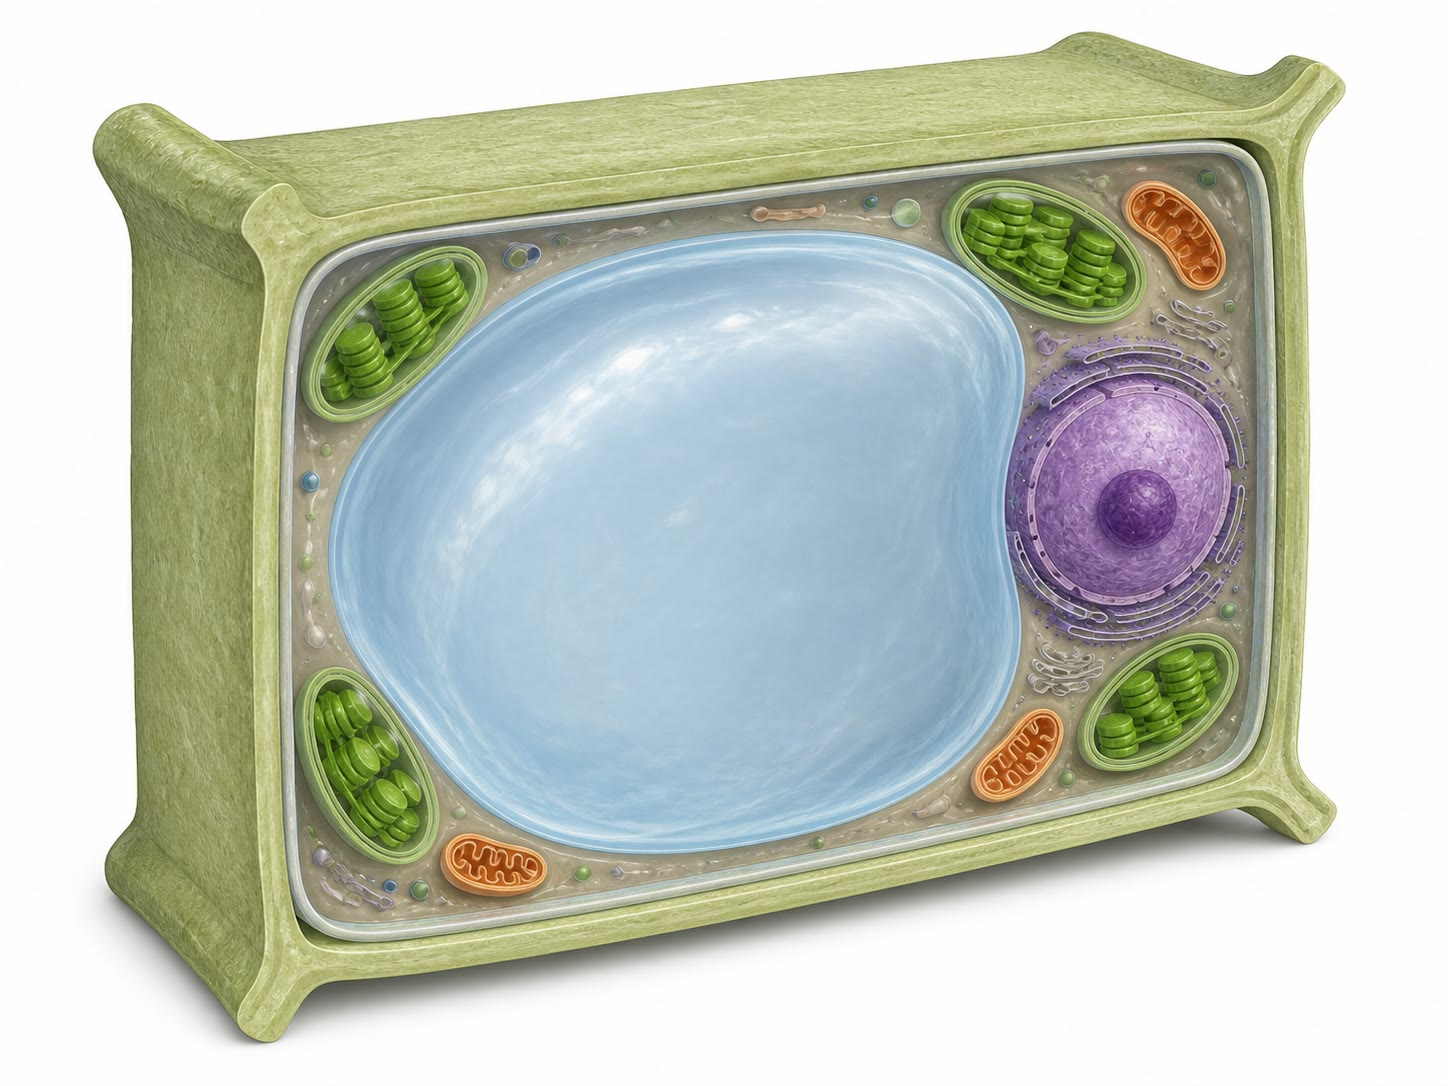
\includegraphics[width=0.52\linewidth]{images/book2/ai/fig-plant-cell-cutaway-v2.jpg}};
  \begin{scope}[x={(img.south east)}, y={(img.north west)},
      every node/.style={font=\small}]
    \draw[omDef, thick] (0.50,0.50) -- (0.50,1.08) node[above] {فجوة مركزية};
    \draw[omDef, thick] (0.10,0.50) -- (-0.03,0.56) node[left] {جدار خلوي};
    \draw[omDef, thick] (0.25,0.73) -- (-0.03,0.84) node[left] {بلاستيدة خضراء};
    \draw[omDef, thick] (0.35,0.17) -- (-0.03,0.12) node[left] {متقدرة};
    \draw[omDef, thick] (0.76,0.47) -- (1.03,0.60) node[right] {نواة};
    \draw[omDef, thick] (0.60,0.13) -- (1.03,0.16) node[right] {سيتوبلازم رقيق};
  \end{scope}
\end{tikzpicture}

{\small \omterm{def:b1:cell-unit-of-life:cell}{خلية} نباتية: الجدار خارج الغشاء، \omterm{def:b1:eukaryotic-cell:plantcell}{والفجوة} تملأ معظم الحجم،
\omterm{def:b1:eukaryotic-cell:plastid}{والبلاستيدات الخضراء} \omterm{def:b1:eukaryotic-cell:mitochondrion}{والمتقدرات} في الطبقة الرقيقة من \omterm{def:b1:cell-unit-of-life:cell}{السيتوبلازم}
بينهما.}
\end{omfigure}

\begin{proposition}[مقارنة الخلية النباتية بالحيوانية]\label{prop:b1:eukaryotic-cell:compare}
لكلتيهما \omterm{def:b1:eukaryotic-cell:nucleus}{نواة} \omterm{def:b1:eukaryotic-cell:endomembrane}{وشبكة إندوبلازمية} \omterm{def:b1:eukaryotic-cell:endomembrane}{وجهاز غولجي} \omterm{def:b1:eukaryotic-cell:mitochondrion}{ومتقدرات} \omterm{def:b1:eukaryotic-cell:peroxisome}{وبيروكسيسومات}
وريبوزومات \omterm{def:b1:eukaryotic-cell:cytoskeleton}{وهيكل خلوي}. وللخلية النباتية جدار سليولوزي، \omterm{def:b1:eukaryotic-cell:plantcell}{وفجوة} كبيرة،
وبلاستيدات، وروابط سيتوبلازمية، ولا مريكزات لها ولا جسيمات حالة
(\omterm{def:b1:eukaryotic-cell:plantcell}{فالفجوة} تهضم)؛ وهي لا تزحف ولا تبتلع، وتنقسم ببناء جدار جديد في
المنتصف. أما \omterm{def:b1:cell-unit-of-life:cell}{الخلية} الحيوانية فلا جدار لها (ولذلك تستطيع أن تغير
شكلها وتزحف وتبلعم)، ولها جسيمات حالة، \omterm{def:b1:eukaryotic-cell:cytoskeleton}{وجسيم مركزي} بمريكزين، وهي
تتواصل عبر وصلات لا عبر روابط سيتوبلازمية؛ وتنقسم بأن تُقرص نصفين.
\end{proposition}

\begin{example}[الامتلاء]\label{ex:b1:eukaryotic-cell:turgor}
\omterm{def:b1:cell-unit-of-life:cell}{خلية} \omterm{def:b1:flowering-plant-organization:organs}{ورقة} تحمل فجوتها \qty{0.3}{mol/L} من المذابات تجذب الماء إلى
أن يدفع الجدار مقابلها بضغط يناهز \qty{0.7}{MPa}، أي سبعة أجواء؛
فتكون \omterm{def:b1:cell-unit-of-life:cell}{الخلية} عندئذ ممتلئة \omterm{def:b1:flowering-plant-organization:organs}{والورقة} متماسكة. وإذا حُرمت الماء فقدت
\omterm{def:b1:eukaryotic-cell:plantcell}{الفجوة} حجمًا وهبط الضغط إلى الصفر وذبلت \omterm{def:b1:flowering-plant-organization:organs}{الورقة} --- والجدار كما هو،
والضغط قد زال (\cref{ch:b1:membranes-transport}). أما \omterm{def:b1:cell-unit-of-life:cell}{خلية} حيوانية
في المحلول نفسه، ولا جدار لها، فكانت لتنفجر ببساطة.
\end{example}

\section{تمارين}

\begin{exercise}[$\star$]\label{exo:b1:eukaryotic-cell:1}
اذكر \omterm{def:b1:cell-unit-of-life:prokeuk}{العضيات} المحدودة بأغشية في \omterm{def:b1:cell-unit-of-life:cell}{خلية} حيوانية وأعطِ الوظيفة الرئيسة
لكل منها في كلمات قليلة.
\end{exercise}

\begin{exercise}[$\star$]\label{exo:b1:eukaryotic-cell:2}
تتبع مسار إنزيم هاضم من تصنيعه إلى القناة، مسميًا كل حجيرة وكيف يمر
البروتين بينها.
\end{exercise}

\begin{exercise}[$\star$]\label{exo:b1:eukaryotic-cell:3}
من شكل ميزانية الأغشية، ما الكسر من غشاء \omterm{def:b1:cell-unit-of-life:cell}{الخلية} الذي هو متقدري
(خارجي مع داخلي)؟ ولماذا كان الغشاء الداخلي أكبر بكثير من الخارجي؟
\end{exercise}

\begin{exercise}[$\star$]\label{exo:b1:eukaryotic-cell:4}
أعطِ ثلاث بنى تملكها \omterm{def:b1:cell-unit-of-life:cell}{الخلية} النباتية ولا تملكها الحيوانية، واثنتين
تملكهما الحيوانية ولا تملكهما النباتية.
\end{exercise}

\begin{exercise}[$\star\star$]\label{exo:b1:eukaryotic-cell:5}
من شكل النبضة والملاحقة، عند أي زمن يبلغ الوسم ذروته في الشبكة، وفي
غولجي، وفي الحبيبات؟ وقدّر زمن العبور من الشبكة إلى الحبيبة والزمن
اللازم قبل أن يُفرز نصف الوسم.
\end{exercise}

\begin{exercise}[$\star\star$]\label{exo:b1:eukaryotic-cell:6}
تُعالَج \omterm{def:b1:cell-unit-of-life:cell}{خلية} بدواء يفكك بلمرة \omterm{def:b1:eukaryotic-cell:cytoskeleton}{الأنيبيبات الدقيقة}. تنبأ بالآثار في
موضع غولجي، وفي حركة الحويصلات، وفي انقسام \omterm{def:b1:cell-unit-of-life:cell}{الخلية}، وفي خفقان
الأهداب.
\end{exercise}

\begin{exercise}[$\star\star$]\label{exo:b1:eukaryotic-cell:7}
أعطِ أربعة شواهد على الأصل البكتيري \omterm{def:b1:eukaryotic-cell:mitochondrion}{للمتقدرات}، وفسّر لماذا لا تستطيع
\omterm{def:b1:eukaryotic-cell:mitochondrion}{المتقدرة} مع ذلك أن تعيش خارج \omterm{def:b1:cell-unit-of-life:cell}{خلية}.
\end{exercise}

\begin{exercise}[$\star\star$]\label{exo:b1:eukaryotic-cell:8}
لمعة \omterm{def:b1:eukaryotic-cell:endomembrane}{الشبكة الإندوبلازمية} «خارج \omterm{def:b1:cell-unit-of-life:cell}{الخلية} من حيث الطوبولوجيا». فسّر
العبارة بتتبع بروتين غشائي تواجه سلاسله السكرية اللمعةَ من الشبكة
إلى الغشاء البلازمي: فأي جهة تواجه السكريات في النهاية؟
\end{exercise}

\begin{exercise}[$\star\star$]\label{exo:b1:eukaryotic-cell:9}
\omterm{def:b1:cell-unit-of-life:cell}{خلية} مفرزة تطلق \qty{2000}{} حبيبة قطرها \qty{1}{\micro m} في اليوم
عبر سطح قمي مساحته \qty{40}{\micro m^2}. احسب الغشاء المضاف في اليوم
وكم مرة يجب أن يُعاد تدوير السطح القمي. فماذا يقتضي هذا؟
\end{exercise}

\begin{exercise}[$\star\star\star$]\label{exo:b1:eukaryotic-cell:10}
في أنبوب اختبار يحوي ريبوزومات وmRNA لبروتين مفرز وحموضًا أمينية،
يكون الناتج سلسلة من \qty{320}{} بقية؛ وبإضافة حويصلات من الشبكة
تظهر سلسلة من \qty{300}{} بقية داخل الحويصلات ولا يهضمها بروتياز
يُضاف بعد ذلك. فسّر كل ملاحظة، وقل ماذا كانت لتفعل طافرة تفتقر إلى
البقايا العشرين الأولى.
\end{exercise}

\begin{exercise}[$\star\star\star$]\label{exo:b1:eukaryotic-cell:11}
\omterm{def:b1:cell-unit-of-life:cell}{خلايا} مريض تفتقر إلى إنزيم حال يهدم دهنًا؛ فيتراكم الدهن في جسيمات
حالة منتفخة وتموت \omterm{def:b1:cell-unit-of-life:cell}{الخلايا}. فسّر بيولوجيا \omterm{def:b1:cell-unit-of-life:cell}{الخلية} في ذلك، وقل لماذا
كان المرض أشد في \omterm{def:b1:cell-unit-of-life:cell}{الخلايا} الأسرع تجديدًا لأغشيتها، واقترح كيف يستطيع
إنزيم يُحقن في الدم أن يبلغ \omterm{def:b1:eukaryotic-cell:endomembrane}{الجسيمات الحالة}.
\end{exercise}

\begin{exercise}[$\star\star\star$]\label{exo:b1:eukaryotic-cell:12}
«\omterm{def:b1:cell-unit-of-life:prokeuk}{الخلية حقيقية النواة} اتحاد من بكتيريا سابقة تجمعها جملة غشائية.»
ناقش في فقرة، موازنًا بين ما تفسره نظرية \omterm{prop:b1:eukaryotic-cell:endosymbiosis}{التعايش الداخلي} وما لا
تفسره (\omterm{def:b1:eukaryotic-cell:nucleus}{النواة}، والشبكة، \omterm{def:b1:eukaryotic-cell:cytoskeleton}{والهيكل الخلوي}).
\end{exercise}

\section{مسألة: الخلية العنبية في البنكرياس}

\begin{problem}[{مسألة نهاية الأسبوع --- خلية تفرز ما يعادل كتلتها من
البروتين كل يوم: ساعة بالادِه، والغشاء الذي عليها أن تعيد تدويره،
والإشارة التي توجه البروتين، وصولًا إلى زمن عبور إنزيم هاضم}]
\label{pb:b1:eukaryotic-cell:1}
\omterm{def:b1:cell-unit-of-life:cell}{الخلية} العنبية البنكرياسية مكعب ضلعه \qty{12}{\micro m}، وجهها القمي
(\qty{144}{\micro m^2}) على القناة ووجهها القاعدي على الدم. وبنكرياس
إنسان كتلته \qty{80}{g} يحمل نحو $\num{8e10}$ \omterm{def:b1:cell-unit-of-life:cell}{خلية} كهذه ويفرز
\qty{10}{g} من البروتين الإنزيمي في اليوم. والحبيبة الإفرازية كرة
قطرها \qty{1}{\micro m} تحمل بروتينًا بتركيز \qty{200}{mg/mL}.
والريبوزومات تضيف \qty{5}{} حموض أمينية في الثانية؛ والإنزيم النموذجي
له \qty{250}{} بقية كتلتها الوسطية \qty{110}{g/mol}.

\medskip
\noindent\textbf{الجزء الأول --- ساعة بالادِه.}
يعطي شكل النبضة والملاحقة في هذا الفصل موضع الوسم بدلالة الزمن.
\begin{enumerate}
  \item لماذا يجب أن تكون النبضة قصيرة وأن تحوي الملاحقة فائضًا
        كبيرًا من الحمض الأميني غير الموسوم؟
  \item اقرأ الزمن الذي يبلغ عنده الوسم ذروته في الشبكة، وفي غولجي،
        وفي الحبيبات.
  \item قدّر زمن العبور من الشبكة إلى غولجي ومن غولجي إلى الحبيبة.
  \item أين يقع الوسم عند \qty{60}{min}، ولماذا غادر بعضه \omterm{def:b1:cell-unit-of-life:cell}{الخلية}
        بينما ما زال معظمه في الحبيبات؟
  \item تُجرى تجربة ثانية عند \qty{15}{\celsius}: فيبقى الوسم في
        الشبكة أكثر من ساعة. فسّر.
\end{enumerate}

\medskip
\noindent\textbf{الجزء الثاني --- كتلة البروتين.}
\begin{enumerate}[resume]
  \item احسب البروتين المفرز لكل \omterm{def:b1:cell-unit-of-life:cell}{خلية} في اليوم، بالبيكوغرام.
  \item احسب حجم حبيبة واحدة وكتلة البروتين التي تحملها.
  \item احسب عدد الحبيبات المطلقة لكل \omterm{def:b1:cell-unit-of-life:cell}{خلية} في اليوم، وفي الدقيقة.
  \item احسب حجم \omterm{def:b1:cell-unit-of-life:cell}{الخلية}، ثم كتلتها بكثافة \qty{1.05}{g/cm^3}. فأي
        كسر من كتلتها تفرزه كل يوم؟
  \item احسب عدد جزيئات الإنزيم في حبيبة واحدة (عدد أفوغادرو
        $\num{6.0e23}$).
  \item احسب الزمن الذي يلزم ريبوزومًا لصنع جزيء إنزيم واحد.
  \item كم ريبوزومًا يجب أن يعمل باستمرار لإنتاج الحصيلة اليومية؟
        قارن مع $\num{4e6}$ ريبوزوم تحويها \omterm{def:b1:cell-unit-of-life:cell}{خلية} كهذه.
\end{enumerate}

\medskip
\noindent\textbf{الجزء الثالث --- الغشاء.}
\begin{enumerate}[resume]
  \item احسب مساحة غشاء حبيبة واحدة.
  \item احسب الغشاء الموصَل إلى الوجه القمي في اليوم بإخراج حبيبات
        السؤال 8.
  \item كم مرة في اليوم تُضاف مساحة الوجه القمي؟ وماذا يجب على
        \omterm{def:b1:cell-unit-of-life:cell}{الخلية} أن تفعل بها، وبأي عملية؟
  \item يأتي غشاء الحبيبة من غولجي، الذي يتلقاه من الشبكة. فإذا كان
        لشبكة \omterm{def:b1:cell-unit-of-life:cell}{الخلية} \qty{20000}{\micro m^2} من الغشاء، فكم يومًا من
        غشاء الحبيبات يعادل ذلك؟ وماذا يقول هذا عن إعادة التدوير
        داخل \omterm{def:b1:eukaryotic-cell:endomembrane}{الجملة الغشائية الداخلية}؟
  \item يحمل الوجه القمي \qty{2000}{} زغيبة قطرها
        \qty{0.1}{\micro m} وطولها \qty{1}{\micro m}. فبأي عامل
        توسّع الوجه البالغ \qty{144}{\micro m^2}؟
\end{enumerate}

\medskip
\noindent\textbf{الجزء الرابع --- العنوان على البروتين.}
\begin{enumerate}[resume]
  \item mRNA لإنزيم يُترجم في أنبوب اختبار بلا أغشية يعطي سلسلة تزيد
        \qty{20}{} بقية عن الإنزيم الموجود في الحبيبات. فأين تقع
        البقايا الزائدة وما هي؟
  \item وبوجود حويصلات من الشبكة يكون الناتج بالطول الصحيح، داخل
        الحويصلات، ومحميًا من بروتياز. فسّر.
  \item والتجربة نفسها مع mRNA لإنزيم عصاري تعطي ناتجًا خارج
        الحويصلات وغير محمي. استنتج.
  \item طفرة تحذف البقايا العشرين. تنبأ بأين ينتهي الإنزيم وماذا يحل
        \omterm{def:b1:cell-unit-of-life:cell}{بالخلية}.
  \item إنزيم آخر يوجد في \omterm{def:b1:eukaryotic-cell:endomembrane}{الجسيمات الحالة} لا في الحبيبات، وهو يحمل
        النوع نفسه من \omterm{prop:b1:eukaryotic-cell:secretory}{تسلسل الإشارة}. فأين على امتداد السبيل يجب أن
        يُتخذ القرار الثاني، وبأي آلية، في الخطوط العامة؟
  \item تُعالَج \omterm{def:b1:cell-unit-of-life:cell}{خلية} بدواء يسد تصنيع ATP. تنبأ بأين يتراكم وسم نبضة
        وملاحقة ولماذا (سببان).
  \item اجمع بين السؤالين 3 و8: في الحالة المستقرة، كم حبيبة تكون
        «في الطريق» بين الشبكة والحبيبة في أي لحظة؟
  \item لخّص النتيجة: زمن العبور من التصنيع إلى الحبيبة، والزمن حتى
        الإفراز، والحبيبات المطلقة في الدقيقة، والكسر من كتلتها الذي
        تفرزه \omterm{def:b1:cell-unit-of-life:cell}{الخلية} يوميًا.
\end{enumerate}
\end{problem}
